\chapter{Quantum Mechanics for Chemists: Model Systems}\label{ch:b3:quantum-model-systems}

Three small flasks stand on a bench, each holding a solution of a cyanine
dye in ethanol: the first is magenta, the second blue, the third a deep
greenish blue that absorbs in the far red. The three molecules are built
alike --- two identical nitrogen-containing rings joined by a chain of
carbon atoms --- and differ only in the length of that chain, by two carbon
atoms at a time. Lengthen the chain and the colour moves to the red. A
chemist of 1949 explained the series with one of the simplest problems of
quantum mechanics: an electron free to move along a line of fixed length,
a ``\omterm{def:b3:quantum-model-systems:box}{particle in a box}''. This chapter sets up the machinery behind that
explanation --- \omterm{def:b3:quantum-model-systems:operator}{operators}, \omterm{def:b3:quantum-model-systems:operator}{eigenvalues}, the \omterm{thm:b3:quantum-model-systems:schrodinger}{Schrödinger equation} --- and
solves the model systems that chemistry uses every day: the box, the
\omterm{def:b3:quantum-model-systems:oscillator}{harmonic oscillator} of a vibrating bond, the \omterm{def:b3:quantum-model-systems:rotor}{rigid rotor} of a turning
molecule, the hydrogen atom, and the barrier that a light particle can
cross without the energy to climb it.

\begin{recall}
The Year 1 volume showed that the energy of an atom is quantised (energy
levels, ground and excited states, the lines of hydrogen) and that a photon
carries $E = h\nu = hc/\lambda$. The Year 2 volume described an electron by
a wavefunction $\psi$ whose square is a probability density, split the
orbitals of hydrogen into radial and angular parts, and counted their nodes;
it took the hydrogen wavefunctions as given. They are derived here, in
section 5. From physics: momentum $p = mv$ and the de Broglie wavelength
$\lambda = h/p$.
\end{recall}

\begin{omfigure}
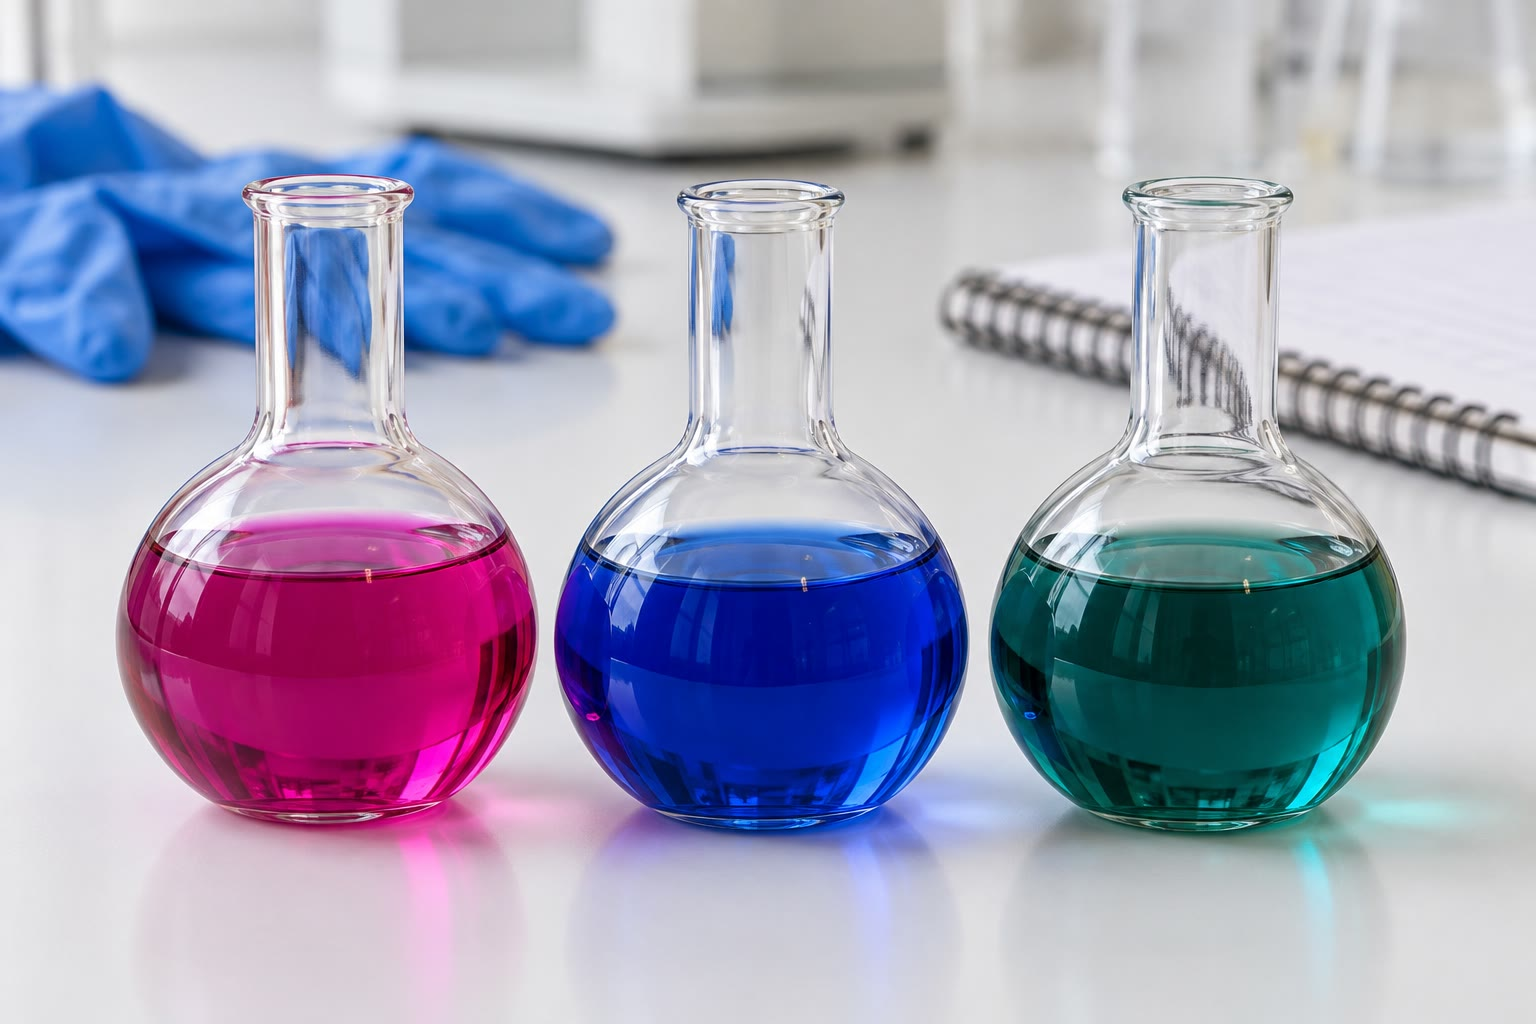
\includegraphics[width=0.62\linewidth]{images/book4/ai/b3-01-dyes.jpg}

{\small Solutions of three cyanine dyes of one family. Each added pair
of carbon atoms in the chain shifts the absorption towards the red.}
\end{omfigure}

\section{Operators, eigenvalues and the Schrödinger equation}

Classical mechanics gives a particle a position and a momentum at each
instant. Quantum mechanics gives it a state, the wavefunction $\psi$, and
replaces each measurable quantity by an operation performed on $\psi$.

\begin{definition}[Operator, eigenfunction, eigenvalue]\label{def:b3:quantum-model-systems:operator}
An \emph{operator}\index{operator} $\hat A$ is a rule that turns a function
into another function: $\hat A f = g$. It is linear if $\hat A(\lambda f +
\mu g) = \lambda\hat Af + \mu\hat Ag$. A non-zero function $f$ such that
$\hat Af = a f$ for a number $a$ is an \emph{eigenfunction}\index{eigenfunction}
of $\hat A$, and $a$ is the corresponding \emph{eigenvalue}\index{eigenvalue}.
\end{definition}

\begin{example}[Two operators of position and momentum]\label{ex:b3:quantum-model-systems:xp}
In one dimension the position \omterm{def:b3:quantum-model-systems:operator}{operator} multiplies by $x$, $\hat x f = xf$,
and the momentum \omterm{def:b3:quantum-model-systems:operator}{operator} differentiates, $\hat p f = -\iu\hbar\,
\dd f/\dd x$, with $\hbar = h/2\pi$. The function $\eu^{\iu kx}$ is an
\omterm{def:b3:quantum-model-systems:operator}{eigenfunction} of $\hat p$ with \omterm{def:b3:quantum-model-systems:operator}{eigenvalue} $\hbar k$: a wave of wavelength
$\lambda = 2\pi/k$ has momentum $h/\lambda$, de Broglie's relation.
The function $\sin kx$ is not an \omterm{def:b3:quantum-model-systems:operator}{eigenfunction} of $\hat p$ (its derivative is
a cosine), but it is one of $\hat p^2 = -\hbar^2\,\dd^2/\dd x^2$, with
\omterm{def:b3:quantum-model-systems:operator}{eigenvalue} $\hbar^2k^2$.
\end{example}

\begin{definition}[Hermitian operator, expectation value]\label{def:b3:quantum-model-systems:hermitian}
Write $\langle f|g\rangle = \int f^*g\,\dd\tau$ for two functions that vanish
at the boundaries of the region. An \omterm{def:b3:quantum-model-systems:operator}{operator} is \emph{Hermitian}\index{Hermitian operator}
if $\langle f|\hat Ag\rangle = \langle \hat Af|g\rangle$ for all such
$f$ and $g$. For a normalised state $\psi$ ($\langle\psi|\psi\rangle = 1$), the
\emph{expectation value}\index{expectation value} of $\hat A$ is
$\langle A\rangle = \langle\psi|\hat A\psi\rangle$: the mean of many
measurements made on identically prepared systems.
\end{definition}

The working rules of quantum chemistry --- its postulates --- can now be
stated in one breath: every measurable quantity is represented by a
\omterm{def:b3:quantum-model-systems:hermitian}{Hermitian operator}; a measurement gives one of its \omterm{def:b3:quantum-model-systems:operator}{eigenvalues}; and if
$\psi$ is an \omterm{def:b3:quantum-model-systems:operator}{eigenfunction} of $\hat A$, every measurement on it gives the
same value, its \omterm{def:b3:quantum-model-systems:operator}{eigenvalue}.

\begin{theorem}[Hermitian operators]\label{thm:b3:quantum-model-systems:hermitian-real}
The \omterm{def:b3:quantum-model-systems:operator}{eigenvalues} of a \omterm{def:b3:quantum-model-systems:hermitian}{Hermitian operator} are real. Two \omterm{def:b3:quantum-model-systems:operator}{eigenfunctions} with
different \omterm{def:b3:quantum-model-systems:operator}{eigenvalues} are orthogonal: $\langle f_1|f_2\rangle = 0$.
\end{theorem}

\begin{proof}
Let $\hat Af = af$. Then $\langle f|\hat Af\rangle = a\langle f|f\rangle$ and
$\langle\hat Af|f\rangle = a^*\langle f|f\rangle$. The \omterm{def:b3:quantum-model-systems:operator}{operator} is \omterm{def:b3:quantum-model-systems:hermitian}{Hermitian},
so the two are equal, and $\langle f|f\rangle > 0$: $a = a^*$. Now let $\hat Af_1
= a_1f_1$ and $\hat Af_2 = a_2f_2$ with $a_1 \ne a_2$, both real. Then
$\langle f_1|\hat Af_2\rangle = a_2\langle f_1|f_2\rangle$ and $\langle\hat Af_1|
f_2\rangle = a_1\langle f_1|f_2\rangle$; their equality gives $(a_2 - a_1)
\langle f_1|f_2\rangle = 0$, hence $\langle f_1|f_2\rangle = 0$.
\end{proof}

A measured value is a real number, which is why observables must be
\omterm{def:b3:quantum-model-systems:hermitian}{Hermitian}; orthogonality is what makes the orbitals of an atom, or the
levels of a box, a clean set of independent states.

\begin{definition}[Commutator]\label{def:b3:quantum-model-systems:commutator}
The \emph{commutator}\index{commutator} of two \omterm{def:b3:quantum-model-systems:operator}{operators} is $[\hat A,\hat B] =
\hat A\hat B - \hat B\hat A$. The \omterm{def:b3:quantum-model-systems:operator}{operators} commute if their commutator is
zero.
\end{definition}

\begin{example}[The canonical commutator]\label{ex:b3:quantum-model-systems:canonical}
For any function $f$, $\hat x\hat pf = -\iu\hbar xf'$ and $\hat p\hat xf =
-\iu\hbar(f + xf')$. The difference is $[\hat x,\hat p]f = \iu\hbar f$, so
$[\hat x,\hat p] = \iu\hbar$: position and momentum do not commute. This
single relation underlies the uncertainty principle and, below, the whole
spectrum of the \omterm{def:b3:quantum-model-systems:oscillator}{harmonic oscillator}.
\end{example}

\begin{proposition}[Commuting operators]\label{prop:b3:quantum-model-systems:commuting}
If $\hat A$ and $\hat B$ commute and $f$ is an \omterm{def:b3:quantum-model-systems:operator}{eigenfunction} of $\hat A$
with a non-degenerate \omterm{def:b3:quantum-model-systems:operator}{eigenvalue} $a$, then $f$ is also an \omterm{def:b3:quantum-model-systems:operator}{eigenfunction} of
$\hat B$.
\end{proposition}

\begin{proof}
$\hat A(\hat Bf) = \hat B\hat Af = a(\hat Bf)$: the function $\hat Bf$ is an
\omterm{def:b3:quantum-model-systems:operator}{eigenfunction} of $\hat A$ with the same \omterm{def:b3:quantum-model-systems:operator}{eigenvalue} $a$, or zero. The
\omterm{def:b3:quantum-model-systems:operator}{eigenvalue} being non-degenerate, $\hat Bf$ is a multiple of $f$, say $bf$.
\end{proof}

The \omterm{def:b3:quantum-model-systems:operator}{operator} of energy is the Hamiltonian. For a particle of mass $m$ in a
potential $V$, the classical energy $p^2/2m + V$ becomes an \omterm{def:b3:quantum-model-systems:operator}{operator}.

\begin{definition}[Hamiltonian operator]\label{def:b3:quantum-model-systems:schrodinger}
The \emph{Hamiltonian operator}\index{Hamiltonian operator} of a particle of
mass $m$ moving in a potential $V(\mathbf r)$ is
\[
\hat H = -\frac{\hbar^2}{2m}\nabla^2 + V(\mathbf r), \qquad \nabla^2 =
\frac{\partial^2}{\partial x^2} + \frac{\partial^2}{\partial y^2} +
\frac{\partial^2}{\partial z^2},
\]
and for several particles, the sum of their kinetic terms and of all their
potential energies.
\end{definition}

\begin{theorem}[The Schrödinger equation]\label{thm:b3:quantum-model-systems:schrodinger}
The states of definite energy of a system --- its stationary states --- are
the \omterm{def:b3:quantum-model-systems:operator}{eigenfunctions} of its Hamiltonian, and its allowed energies are the
\omterm{def:b3:quantum-model-systems:operator}{eigenvalues}:
\[
\hat H\psi = E\psi,
\]
the time-independent \emph{Schrödinger equation}\index{Schrödinger equation}.
An acceptable $\psi$ is single-valued, continuous, and
square-integrable (it can be normalised).
\end{theorem}
\begin{proof}[Status]
This is a postulate, justified by its consequences: the levels of every
system solved below agree with spectroscopy. The time-dependent equation,
of which this is the stationary case, belongs to physics.
\end{proof}

The boundary conditions do the quantising: a differential equation has
solutions for every $E$, but only a discrete set of them stays finite and
continuous. Chemistry is then a matter of choosing a potential, solving,
and reading the \omterm{def:b3:quantum-model-systems:operator}{eigenvalues}.

\begin{method}[Solving a one-dimensional model]\label{met:b3:quantum-model-systems:one-dimensional}
\begin{enumerate}
  \item Write the potential $V(x)$ and the Hamiltonian; split space into
        regions where $V$ is simple.
  \item Solve $-\frac{\hbar^2}{2m}\psi'' + V\psi = E\psi$ in each region: sines
        and cosines where $E > V$, real exponentials where $E < V$.
  \item Impose the conditions: $\psi = 0$ where $V$ is infinite; $\psi$
        and $\psi'$ continuous at a finite step; $\psi \to 0$ at infinity.
  \item The conditions are met only for certain $E$: these are the levels.
  \item Normalise each \omterm{def:b3:quantum-model-systems:operator}{eigenfunction}; count its nodes as a check (the
        $n$-th level of a one-dimensional problem has $n - 1$ nodes).
\end{enumerate}
\end{method}

\section{The particle in a box}

\begin{definition}[Particle in a box, free-electron model]\label{def:b3:quantum-model-systems:box}
A \emph{particle in a box}\index{particle in a box} moves freely ($V = 0$)
between $x = 0$ and $x = L$ and cannot leave ($V = \infty$ outside). The
\emph{free-electron model}\index{free-electron model} of a conjugated
molecule treats its $\pi$ electrons as independent particles in a box whose
length is that of the conjugated chain.
\end{definition}

\begin{theorem}[Levels of the box]\label{thm:b3:quantum-model-systems:box}
The levels and normalised \omterm{def:b3:quantum-model-systems:operator}{eigenfunctions} of a particle of mass $m$ in a box
of length $L$ are
\[
E_n = \frac{n^2h^2}{8mL^2}, \qquad \psi_n(x) = \sqrt{\frac2L}\,\sin\frac{n\pi
x}{L}, \qquad n = 1, 2, 3, \dots
\]
\end{theorem}

\begin{proof}
Inside, $\psi'' = -k^2\psi$ with $k^2 = 2mE/\hbar^2$, so $\psi = A\sin kx +
B\cos kx$. Outside $\psi = 0$ and continuity gives $\psi(0) = 0$, hence $B =
0$, and $\psi(L) = 0$, hence $\sin kL = 0$ with $A \ne 0$: $kL = n\pi$, $n$ a
positive integer ($n = 0$ gives $\psi = 0$; negative $n$ repeat the same
functions). Then $E = \hbar^2k^2/2m = n^2\pi^2\hbar^2/2mL^2 = n^2h^2/8mL^2$.
Finally $\int_0^L A^2\sin^2(n\pi x/L)\,\dd x = A^2L/2 = 1$ gives $A =
\sqrt{2/L}$.
\end{proof}

Three features carry over to every bound system: the lowest energy is not
zero (the particle can never be at rest), the levels spread apart as $n$
grows, and they crowd together as the box grows ($E \propto 1/L^2$): a
large box is nearly classical.

\begin{omfigure}
\begin{tikzpicture}
\begin{axis}[width=0.5\linewidth, height=6.4cm, xmin=-0.08, xmax=1.08,
  ymin=0, ymax=18.4, axis lines=left, xtick={0,1}, xticklabels={$0$,$L$},
  ytick={1,4,9,16}, yticklabels={$E_1$,$4E_1$,$9E_1$,$16E_1$},
  tick label style={font=\small}, xlabel={$x$}, title={\small $\psi_n$}]
\foreach \n in {1,4,9,16}{\addplot[gray!50, dashed, domain=0:1] {\n};}
\addplot[omDef, thick] table[x=x, y=p1] {figdata/out/bachelor-3-particle-in-box.dat};
\addplot[omDef, thick] table[x=x, y=p2] {figdata/out/bachelor-3-particle-in-box.dat};
\addplot[omDef, thick] table[x=x, y=p3] {figdata/out/bachelor-3-particle-in-box.dat};
\addplot[omDef, thick] table[x=x, y=p4] {figdata/out/bachelor-3-particle-in-box.dat};
\draw[very thick] (axis cs:0,0) -- (axis cs:0,18.4) (axis cs:1,0) -- (axis cs:1,18.4);
\end{axis}
\end{tikzpicture}\hspace{0.5em}%
\begin{tikzpicture}
\begin{axis}[width=0.5\linewidth, height=6.4cm, xmin=-0.08, xmax=1.08,
  ymin=0, ymax=18.4, axis lines=left, xtick={0,1}, xticklabels={$0$,$L$},
  ytick={1,4,9,16}, yticklabels={$n=1$,$n=2$,$n=3$,$n=4$},
  tick label style={font=\small}, xlabel={$x$}, title={\small $|\psi_n|^2$}]
\foreach \n in {1,4,9,16}{\addplot[gray!50, dashed, domain=0:1] {\n};}
\addplot[omThm, thick] table[x=x, y=d1] {figdata/out/bachelor-3-particle-in-box.dat};
\addplot[omThm, thick] table[x=x, y=d2] {figdata/out/bachelor-3-particle-in-box.dat};
\addplot[omThm, thick] table[x=x, y=d3] {figdata/out/bachelor-3-particle-in-box.dat};
\addplot[omThm, thick] table[x=x, y=d4] {figdata/out/bachelor-3-particle-in-box.dat};
\draw[very thick] (axis cs:0,0) -- (axis cs:0,18.4) (axis cs:1,0) -- (axis cs:1,18.4);
\end{axis}
\end{tikzpicture}

{\small The first four levels of a \omterm{def:b3:quantum-model-systems:box}{particle in a box}, each function drawn on
its own level (dashed). Left: $\psi_n$, with $n - 1$ nodes inside the box.
Right: the probability density $|\psi_n|^2$.}
\end{omfigure}

\begin{proposition}[The cubic box]\label{prop:b3:quantum-model-systems:box-3d}
In a cubic box of side $L$, $\psi = \psi_{n_x}(x)\psi_{n_y}(y)\psi_{n_z}(z)$ and
$E = (n_x^2 + n_y^2 + n_z^2)\,h^2/8mL^2$. Distinct triples with the same sum
of squares give the same energy.
\end{proposition}

\begin{proof}
With $V = 0$ inside, $\hat H$ is a sum of three one-dimensional \omterm{def:b3:quantum-model-systems:operator}{operators},
one per coordinate. The product of three one-dimensional \omterm{def:b3:quantum-model-systems:operator}{eigenfunctions} is
an \omterm{def:b3:quantum-model-systems:operator}{eigenfunction} of the sum, with the sum of the three \omterm{def:b3:quantum-model-systems:operator}{eigenvalues}; it
vanishes on every face, as required.
\end{proof}

\begin{definition}[Degenerate levels]\label{def:b3:quantum-model-systems:degenerate}
Linearly independent \omterm{def:b3:quantum-model-systems:operator}{eigenfunctions} with the same \omterm{def:b3:quantum-model-systems:operator}{eigenvalue} are
\emph{degenerate levels}\index{degenerate levels}; their number is the
\emph{degeneracy}\index{degeneracy} $g$ of that energy.
\end{definition}

\begin{example}[Degeneracy and symmetry]\label{ex:b3:quantum-model-systems:cube}
The level $n_x^2 + n_y^2 + n_z^2 = 6$ of the cube comes from $(2,1,1)$,
$(1,2,1)$ and $(1,1,2)$: $g = 3$. Stretch the box slightly along $z$ and the
third function moves away from the other two: the \omterm{def:b3:quantum-model-systems:degenerate}{degeneracy} came from
the symmetry of the cube. The same link between symmetry and \omterm{def:b3:quantum-model-systems:degenerate}{degeneracy}
organises \cref{ch:b3:point-groups,ch:b3:group-theory-applied}.
\end{example}

\subsection*{Conjugated dyes}

In a symmetric cyanine dye, a chain of $j$ atoms joins the two nitrogens
(\(j = 5\), 7, 9 for the three dyes of the opening scene), and its $\pi$ electrons
are delocalised along it. A chain of $j$ atoms carries $N = j + 1$ $\pi$
electrons: one per carbon, plus the lone pair of one nitrogen shared over
the whole cation.

\begin{proposition}[Free-electron absorption wavelength]\label{prop:b3:quantum-model-systems:free-electron}
If $N$ $\pi$ electrons (an even number) fill the levels of a box of length $L$,
two per level, the longest-wavelength absorption, from the highest filled
level $n = N/2$ to the next, is at
\[
\lambda = \frac{8mcL^2}{h(N+1)}.
\]
\end{proposition}

\begin{proof}
$\Delta E = E_{N/2+1} - E_{N/2} = [(N/2+1)^2 - (N/2)^2]\,h^2/8mL^2 =
(N+1)\,h^2/8mL^2$, and $\lambda = hc/\Delta E$.
\end{proof}

\begin{example}[The bare box fails, an extended box works]\label{ex:b3:quantum-model-systems:dyes}
% ledger: uvvis:cyanine, uvvis:carbocyanine, uvvis:dicarbocyanine, geo:C6H6.rCC
Take each bond of the chain equal to the C--C bond of benzene,
$l = \qty{139.7}{pm}$, so that the bare chain measures $(j - 1)l$. For the
three dyes ($N = 6$, 8, 10) the formula gives 147, 257 and 374 nm, far
below the measured maxima, 524, 603 and 711 nm in ethanol. The electrons
are not stopped at the nitrogens: they spread into the rings. Extend the
box by a length $\delta$ at each end and fit $\delta$ on the middle dye:
$\delta = \qty{222}{pm}$, about one and a half bonds. The same $\delta$ then
predicts 474 and 732 nm for the other two, within 10\,\% and 3\,\%. A single
adjustable length explains a family of colours (figure below; the numbers are
computed in the figure's script).
\end{example}

\begin{omfigure}
\begin{tikzpicture}
\begin{axis}[width=0.5\linewidth, height=5.6cm, xmin=4, xmax=10,
  ymin=0, ymax=850, xtick={5,7,9}, axis lines=left,
  xlabel={atoms $j$ in the chain}, ylabel={$\lambda_{\max}$ / nm},
  legend cell align=left, legend style={font=\small, at={(1.03,0.5)}, anchor=west, draw=none},
  tick label style={font=\small}, label style={font=\small}]
\addplot[only marks, mark=*, omThm] table[x=j, y=measured] {figdata/out/bachelor-3-particle-in-box-dyes.dat};
\addlegendentry{measured (ethanol)}
\addplot[omDef, thick, mark=square*] table[x=j, y=fitted] {figdata/out/bachelor-3-particle-in-box-dyes.dat};
\addlegendentry{box extended by $\delta = 222$ pm}
\addplot[gray, dashed, mark=triangle*] table[x=j, y=bare] {figdata/out/bachelor-3-particle-in-box-dyes.dat};
\addlegendentry{bare chain}
\end{axis}
\end{tikzpicture}

{\small Absorption maxima of the three cyanine dyes against the
\omterm{def:b3:quantum-model-systems:box}{free-electron model}: the bare chain, and the box extended by $\delta$ at
each end, $\delta$ fitted on the middle dye.}
\end{omfigure}

\begin{inthelab}[Measuring a dye series]
The three dyes are weighed (a few milligrams), dissolved in ethanol and
diluted until the absorbance at the maximum lies between 0.3 and 1. The
spectrum of each is recorded between 400 and 800 nm in a 1 cm cuvette
against a blank of pure ethanol, and $\lambda_{\max}$ read at the top of the
main band. Cyanine dyes are stained and irritant solids: gloves, and
weighing in a fume hood.
\end{inthelab}

\section{The harmonic oscillator}

Near the bottom of any smooth potential well, $V \approx \frac12 k(x - x_e)^2$:
small vibrations of a bond, of an atom in a crystal, of a molecule in a
cage are all approximately harmonic.

\begin{definition}[Harmonic oscillator, force constant, reduced mass, zero-point energy]\label{def:b3:quantum-model-systems:oscillator}
A \emph{harmonic oscillator}\index{harmonic oscillator} is a particle of
mass $m$ in the potential $V = \frac12 kx^2$; $k$ is the \emph{force
constant}\index{force constant}, and $\omega = \sqrt{k/m}$ its classical
angular frequency. A diatomic molecule of atomic masses $m_1$, $m_2$
vibrates as one particle of \emph{reduced mass}\index{reduced mass}
$\mu = m_1m_2/(m_1 + m_2)$ in the potential of its bond. The energy of the
lowest level of an oscillator is its \emph{zero-point energy}\index{zero-point energy}.
\end{definition}

\begin{definition}[Ladder operators]\label{def:b3:quantum-model-systems:ladder}
With $x_0 = \sqrt{\hbar/m\omega}$, the \emph{ladder operators}\index{ladder operators}
are
\[
\hat a = \frac{1}{\sqrt2}\Big(\frac{\hat x}{x_0} + \frac{\iu x_0\hat p}{\hbar}\Big),
\qquad \hat a^\dagger = \frac{1}{\sqrt2}\Big(\frac{\hat x}{x_0} -
\frac{\iu x_0\hat p}{\hbar}\Big).
\]
\end{definition}

\begin{theorem}[Levels of the harmonic oscillator]\label{thm:b3:quantum-model-systems:oscillator}
The levels of a \omterm{def:b3:quantum-model-systems:oscillator}{harmonic oscillator} are
\[
E_v = \big(v + \tfrac12\big)\hbar\omega = \big(v + \tfrac12\big)h\nu, \qquad v =
0, 1, 2, \dots,
\]
equally spaced by $h\nu$, with the \omterm{def:b3:quantum-model-systems:oscillator}{zero-point energy} $\frac12h\nu$.
\end{theorem}

\begin{proof}
From $[\hat x,\hat p] = \iu\hbar$ one computes $[\hat a,\hat a^\dagger] = 1$ and
$\hat H = \hbar\omega(\hat a^\dagger\hat a + \frac12)$. Write $\hat N =
\hat a^\dagger\hat a$. Then $[\hat N,\hat a] = -\hat a$ and $[\hat N,\hat
a^\dagger] = \hat a^\dagger$: if $\hat N\psi = \nu\psi$, then $\hat N(\hat
a\psi) = (\nu - 1)\hat a\psi$ and $\hat N(\hat a^\dagger\psi) = (\nu + 1)\hat
a^\dagger\psi$; $\hat a$ lowers the \omterm{def:b3:quantum-model-systems:operator}{eigenvalue} by one, $\hat a^\dagger$ raises
it. But $\nu = \langle\psi|\hat a^\dagger\hat a\psi\rangle/\langle\psi|\psi
\rangle = \|\hat a\psi\|^2/\|\psi\|^2 \ge 0$: the descent must stop, which
happens only on a function with $\hat a\psi_0 = 0$, of \omterm{def:b3:quantum-model-systems:operator}{eigenvalue} $\nu = 0$.
The \omterm{def:b3:quantum-model-systems:operator}{eigenvalues} of $\hat N$ are therefore $v = 0, 1, 2, \dots$, and those of
$\hat H$ are $(v + \frac12)\hbar\omega$.
\end{proof}

\begin{proposition}[The first wavefunctions]\label{prop:b3:quantum-model-systems:oscillator-functions}
In the reduced coordinate $y = x/x_0$,
\[
\psi_0 \propto \eu^{-y^2/2}, \quad \psi_1 \propto 2y\,\eu^{-y^2/2}, \quad
\psi_2 \propto (4y^2 - 2)\eu^{-y^2/2}, \quad \psi_3 \propto (8y^3 -
12y)\eu^{-y^2/2},
\]
the Hermite polynomials times a Gaussian. $\psi_v$ is even for even $v$,
odd for odd $v$.
\end{proposition}

\begin{proof}
$\hat a\psi_0 = 0$ reads $y\psi_0 + \dd\psi_0/\dd y = 0$, whose solution is the
Gaussian. Each next function is $\hat a^\dagger$ applied to the previous one,
$\hat a^\dagger = \frac{1}{\sqrt2}(y - \dd/\dd y)$, which multiplies the
polynomial by $2y$ and subtracts its derivative: $1 \to 2y \to 4y^2 - 2 \to
8y^3 - 12y$ (up to factors). Changing $y$ into $-y$ changes the sign of $y$
and of $\dd/\dd y$, so $\hat a^\dagger$ flips the parity at each step.
\end{proof}

\begin{omfigure}
\begin{tikzpicture}
\begin{axis}[width=0.66\linewidth, height=6.6cm, xmin=-4, xmax=4, ymin=0,
  ymax=4.6, axis lines=left, xlabel={$y = x/x_0$},
  ylabel={energy / $\hbar\omega$}, ytick={0.5,1.5,2.5,3.5},
  tick label style={font=\small}, label style={font=\small}]
\addplot[black, thick] table[x=y, y=V] {figdata/out/bachelor-3-harmonic-oscillator.dat};
\foreach \v in {0.5,1.5,2.5,3.5}{\addplot[gray!50, dashed, domain=-4:4] {\v};}
\addplot[omDef, thick] table[x=y, y=p0] {figdata/out/bachelor-3-harmonic-oscillator.dat};
\addplot[omDef, thick] table[x=y, y=p1] {figdata/out/bachelor-3-harmonic-oscillator.dat};
\addplot[omDef, thick] table[x=y, y=p2] {figdata/out/bachelor-3-harmonic-oscillator.dat};
\addplot[omDef, thick] table[x=y, y=p3] {figdata/out/bachelor-3-harmonic-oscillator.dat};
\addplot[only marks, mark=*, mark size=1.6pt, omThm] coordinates {(-1,0.5) (1,0.5)};
\node[omThm, font=\small, anchor=west] at (axis cs:2.0,0.2) {turning points};
\draw[omThm, ->, thin] (axis cs:2.0,0.2) -- (axis cs:1.08,0.47);
\end{axis}
\end{tikzpicture}

{\small The harmonic potential, its first four levels and wavefunctions,
each drawn on its level. The wavefunctions reach beyond the classical
turning points ($y = \pm1$ for $v = 0$, red dots), where a classical
particle would stop.}
\end{omfigure}

\begin{example}[Zero-point energies of \ce{H2} and \ce{D2}]\label{ex:b3:quantum-model-systems:zpe}
% ledger: diat:H2.we, diat:D2.we
The harmonic wavenumbers are $\tilde\omega_e = \qty{4401.2}{cm^{-1}}$ for
\ce{H2} and \qty{3115.5}{cm^{-1}} for \ce{D2}, in the ratio $1.413$, close to
$\sqrt2$: same bond and \omterm{def:b3:quantum-model-systems:oscillator}{force constant}, doubled \omterm{def:b3:quantum-model-systems:oscillator}{reduced mass}. The harmonic
zero-point energies are half these, 2200.6 and \qty{1557.8}{cm^{-1}},
\qty{26.3}{kJ/mol} and \qty{18.6}{kJ/mol}. A molecule can never lose this
energy; the difference between isotopes is the source of the isotope effects
of \cref{ch:b3:statistical-thermo-applied,ch:b3:rate-theories}.
\end{example}

\section{The rigid rotor}

A diatomic molecule also turns about its centre of mass. Treated as two
masses at a fixed distance $r$, it is a \omterm{def:b3:quantum-model-systems:rotor}{rigid rotor} of moment of inertia
$I = \mu r^2$, the \omterm{def:b3:quantum-model-systems:oscillator}{reduced mass} at distance $r$ from the axis.

\begin{definition}[Rigid rotor, spherical harmonics]\label{def:b3:quantum-model-systems:rotor}
A \emph{rigid rotor}\index{rigid rotor} is a body of fixed shape turning
freely; for a linear molecule, $\hat H = \hat L^2/2I$, where $\hat L^2$ is the
\omterm{def:b3:quantum-model-systems:operator}{operator} of the square of the angular momentum. Its \omterm{def:b3:quantum-model-systems:operator}{eigenfunctions}, which
depend only on the angles $\theta$ and $\phi$, are the \emph{spherical
harmonics}\index{spherical harmonics} $Y_{l,m}(\theta,\phi)$, labelled by $l =
0, 1, 2, \dots$ and $m = -l, \dots, l$; for a molecule $l$ is written $J$.
\end{definition}

The rotor on a ring (rotation in a plane, about a fixed axis) is solved
first; it holds the essence.

\begin{theorem}[The ring]\label{thm:b3:quantum-model-systems:ring}
A particle of moment of inertia $I$ turning in a plane has levels
$E_m = m^2\hbar^2/2I$ with $m = 0, \pm1, \pm2, \dots$; every level but $m = 0$
is doubly degenerate.
\end{theorem}

\begin{proof}
The only coordinate is the angle $\phi$, and $\hat H = -(\hbar^2/2I)\,
\dd^2/\dd\phi^2$. The solutions of $\psi'' = -(2IE/\hbar^2)\psi$ are $\eu^{\iu
m\phi}$ with $m^2 = 2IE/\hbar^2$. A single-valued function must take the same
value at $\phi$ and $\phi + 2\pi$: $\eu^{2\pi\iu m} = 1$, so $m$ is an integer.
The functions with $m$ and $-m$ have the same energy and are independent.
\end{proof}

\begin{theorem}[Levels of the rigid rotor]\label{thm:b3:quantum-model-systems:rotor}
$\hat L^2Y_{J,m} = J(J+1)\hbar^2\,Y_{J,m}$ and $\hat L_zY_{J,m} = m\hbar\,
Y_{J,m}$, so the levels of a linear \omterm{def:b3:quantum-model-systems:rotor}{rigid rotor} are
\[
E_J = \frac{\hbar^2}{2I}\,J(J+1), \qquad J = 0, 1, 2, \dots,
\]
each with \omterm{def:b3:quantum-model-systems:degenerate}{degeneracy} $g_J = 2J + 1$.
\end{theorem}
\admitted

The general proof, by \omterm{def:b3:quantum-model-systems:ladder}{ladder operators} for angular momentum, is treated in
more advanced courses; here is a check. In spherical coordinates,
\[
\hat L^2 = -\hbar^2\Big[\frac{1}{\sin\theta}\frac{\partial}{\partial\theta}
\Big(\sin\theta\frac{\partial}{\partial\theta}\Big) +
\frac{1}{\sin^2\theta}\frac{\partial^2}{\partial\phi^2}\Big].
\]
For $Y_{1,0} \propto \cos\theta$, the bracket is $\frac{1}{\sin\theta}(-2\sin\theta
\cos\theta) = -2\cos\theta$, so $\hat L^2Y_{1,0} = 2\hbar^2Y_{1,0} = 1(1+1)\hbar^2
Y_{1,0}$. For $Y_{1,\pm1} \propto \sin\theta\,\eu^{\pm\iu\phi}$ the same
computation gives $2\hbar^2$ again, and $\hat L_z = -\iu\hbar\,\partial/\partial
\phi$ gives $\pm\hbar$.

\begin{proposition}[Real spherical harmonics]\label{prop:b3:quantum-model-systems:real-harmonics}
For $l = 1$, the combinations $Y_{1,0}$, $(Y_{1,-1} - Y_{1,1})/\sqrt2$ and
$\iu(Y_{1,-1} + Y_{1,1})/\sqrt2$ are real and proportional to $z/r$, $x/r$ and
$y/r$; for $l = 2$ the same construction gives functions proportional to
$(3z^2 - r^2)$, $xz$, $yz$, $xy$ and $x^2 - y^2$, divided by $r^2$.
\end{proposition}

\begin{proof}
$Y_{1,\pm1} \propto \mp\sin\theta\,\eu^{\pm\iu\phi}$ with the usual sign
convention, so their difference over $\sqrt2$ is $\propto\sin\theta\cos\phi =
x/r$ and the $\iu$-weighted sum $\propto\sin\theta\sin\phi = y/r$;
$\cos\theta = z/r$. Each combination of degenerate \omterm{def:b3:quantum-model-systems:operator}{eigenfunctions} is still an
\omterm{def:b3:quantum-model-systems:operator}{eigenfunction} of $\hat L^2$ (with the same $l$), though no longer of $\hat
L_z$. The $l = 2$ case is the same algebra with $\sin^2\theta\,\eu^{\pm2\iu\phi}$
and $\sin\theta\cos\theta\,\eu^{\pm\iu\phi}$.
\end{proof}

These are the angular parts of the $p$ and $d$ orbitals drawn in the Year
2 volume: their names $p_x$, $d_{xy}$, $d_{z^2}$ are the Cartesian forms just
found.

\begin{omfigure}
\begin{tikzpicture}[font=\small]
  \draw[->] (0,-0.2) -- (0,5.4) node[above] {$E/(\hbar^2/2I)$};
  \foreach \J/\E/\g in {0/0/1,1/2/3,2/6/5,3/12/7}{
    \pgfmathsetmacro{\y}{0.4*\E+0.1}
    \draw[omstate] (0.6,\y) -- (3.0,\y);
    \node[anchor=east] at (0.55,\y) {$\E$};
    \node[anchor=west] at (3.1,\y) {$J = \J$, \ $g = \g$};
  }
  \draw[<->, omThm] (2.4,0.9) -- (2.4,2.5) node[midway, left] {$4$};
  \draw[<->, omThm] (1.4,0.1) -- (1.4,0.9) node[midway, left] {$2$};
\end{tikzpicture}

{\small The first levels of a linear \omterm{def:b3:quantum-model-systems:rotor}{rigid rotor}, $E_J = J(J+1)\,\hbar^2/2I$,
with their degeneracies $2J + 1$. The gaps grow as $2(J+1)$: the reason
for the evenly spaced lines of \cref{ch:b3:rovibrational-spectroscopy}.}
\end{omfigure}

\begin{example}[Rotational levels of \ce{HCl}]\label{ex:b3:quantum-model-systems:hcl}
% ledger: diat:HCl.Be
Spectroscopists write $E_J = hcB\,J(J+1)$ with the rotational constant $B =
\hbar/(4\pi cI)$ in wavenumbers. For \ce{H^{35}Cl}, $B = \qty{10.593}{cm^{-1}}$:
the first levels lie at 0, 21.19, 63.56 and \qty{127.12}{cm^{-1}}, all well
below the thermal energy at room temperature, $kT/hc = \qty{207}{cm^{-1}}$.
Many rotational levels are populated; only one vibrational level is
($\tilde\omega_e = \qty{2991}{cm^{-1}}$).
\end{example}

\section{The hydrogen atom and tunnelling}

\subsection*{The hydrogen atom, solved}

An electron of charge $-e$ around a nucleus of charge $+e$ has $V = -e^2/
4\pi\varepsilon_0r$. With the \omterm{def:b3:quantum-model-systems:oscillator}{reduced mass} $\mu$ of electron and proton,
\[
\hat H = -\frac{\hbar^2}{2\mu}\nabla^2 - \frac{e^2}{4\pi\varepsilon_0r},\qquad
\nabla^2 = \frac{1}{r^2}\frac{\partial}{\partial r}\Big(r^2\frac{\partial}{
\partial r}\Big) - \frac{\hat L^2}{\hbar^2r^2}.
\]
The angular part of $\nabla^2$ is the rotor \omterm{def:b3:quantum-model-systems:operator}{operator}: the solutions
separate as $\psi = R(r)\,Y_{l,m}(\theta,\phi)$, and $R$ obeys the radial
equation
\[
-\frac{\hbar^2}{2\mu}\frac{1}{r^2}\frac{\dd}{\dd r}\Big(r^2\frac{\dd R}{\dd r}
\Big) + \Big[\frac{l(l+1)\hbar^2}{2\mu r^2} - \frac{e^2}{4\pi\varepsilon_0r}
\Big]R = ER.
\]
The rotation adds a centrifugal term $l(l+1)\hbar^2/2\mu r^2$ that keeps
electrons with $l > 0$ away from the nucleus.

\begin{theorem}[Levels of the hydrogen atom]\label{thm:b3:quantum-model-systems:hydrogen}
The bound levels of a hydrogen-like atom of nuclear charge $Ze$ are
\[
E_n = -\frac{\mu}{m_e}\,\frac{Z^2hcR_\infty}{n^2}, \qquad n = 1, 2, \dots,
\quad hcR_\infty = \frac{m_ee^4}{8\varepsilon_0^2h^2},
\]
with $l = 0, \dots, n - 1$; the $1s$ and $2p$ radial functions are $R_{10}
\propto \eu^{-Zr/a}$ and $R_{21} \propto r\,\eu^{-Zr/2a}$, with $a =
(m_e/\mu)a_0$.
\end{theorem}

\begin{proof}[Partial proof]
Take $Z = 1$ and try $R = \eu^{-r/a}$ with $l = 0$. Then $R' = -R/a$ and
$\frac{1}{r^2}(r^2R')' = R/a^2 - 2R/(ar)$. The radial equation becomes
$-\frac{\hbar^2}{2\mu}\big(\frac{1}{a^2} - \frac{2}{ar}\big) - \frac{e^2}{4\pi
\varepsilon_0r} = E$ for all $r$: the terms in $1/r$ cancel if $a =
4\pi\varepsilon_0\hbar^2/\mu e^2$, and then $E = -\hbar^2/2\mu a^2 = -\mu
e^4/8\varepsilon_0^2h^2$, the $n = 1$ level. With $R = r\eu^{-r/b}$ and $l = 1$,
the same substitution leaves terms in $1/r^2$ (which cancel against the
centrifugal term), in $1/r$ (which cancel if $b = 2a$) and a constant, $E =
-\hbar^2/2\mu b^2$, one quarter of the previous: the $n = 2$ level. The general
case, a polynomial times $\eu^{-r/na}$ whose series must terminate to stay
normalisable, is treated in more advanced courses.
\end{proof}

\begin{omfigure}
\begin{tikzpicture}
\begin{axis}[width=0.66\linewidth, height=5.4cm, xmin=0, xmax=12,
  ymin=-0.15, ymax=1.05, axis lines=left, samples=160, domain=0:12,
  xlabel={$r/a$}, ylabel={$R(r)$, scaled},
  legend cell align=left, legend style={font=\small, draw=none}, tick label style={font=\small},
  label style={font=\small}]
\addplot[omDef, thick] {exp(-x)}; \addlegendentry{$R_{10} \propto \eu^{-r/a}$}
\addplot[omThm, thick] {(1-x/2)*exp(-x/2)}; \addlegendentry{$R_{20} \propto (1 - r/2a)\eu^{-r/2a}$}
\addplot[omProp, thick] {0.5*x*exp(-x/2)/exp(-1)}; \addlegendentry{$R_{21} \propto r\,\eu^{-r/2a}$}
\addplot[gray, dashed] {0};
\end{axis}
\end{tikzpicture}

{\small Radial functions of the hydrogen atom, from the solutions above
(each scaled to a maximum near 1). $R_{20}$ has one radial node at $r = 2a$;
$R_{21}$ vanishes at the nucleus, pushed out by the centrifugal term.}
\end{omfigure}

\begin{example}[The ionisation energy of hydrogen]\label{ex:b3:quantum-model-systems:ie}
% ledger: const:RyhcEV, const:me, const:mp
$hcR_\infty = \qty{13.6057}{eV}$ and $\mu/m_e = 1/(1 + m_e/m_p) = 0.999456$, so
$-E_1 = \qty{13.598}{eV}$: the measured ionisation energy of hydrogen, to the
last digit given in the Year 1 volume. The \omterm{def:b3:quantum-model-systems:oscillator}{reduced mass} changes the fourth
significant figure.
\end{example}

\subsection*{Tunnelling}

\begin{definition}[Tunnelling, transmission probability]\label{def:b3:quantum-model-systems:tunnelling}
\emph{Tunnelling}\index{tunnelling} is the passage of a particle through a
region where its energy is lower than the potential energy, forbidden in
classical mechanics. The \emph{transmission probability}\index{transmission probability}
$T$ of a barrier is the fraction of incident particles found
beyond it.
\end{definition}

\begin{proposition}[Thin and thick barriers]\label{prop:b3:quantum-model-systems:barrier}
Inside a barrier of height $V_0 > E$, $\psi$ is a combination of
$\eu^{\pm\kappa x}$ with $\kappa = \sqrt{2m(V_0 - E)}/\hbar$. For a rectangular
barrier of width $a$,
\[
T = \Big[1 + \frac{\sinh^2(\kappa a)}{4\varepsilon(1-\varepsilon)}\Big]^{-1},
\qquad \varepsilon = \frac{E}{V_0},
\]
and for a thick barrier ($\kappa a \gg 1$), $T \approx 16\varepsilon(1-\varepsilon)
\,\eu^{-2\kappa a}$.
\end{proposition}

\begin{proof}[Partial proof]
In the barrier the \omterm{thm:b3:quantum-model-systems:schrodinger}{Schrödinger equation} reads $\psi'' = \kappa^2\psi$, whose
solutions are the two exponentials. Matching $\psi$ and $\psi'$ at the two
walls with the waves $\eu^{\pm\iu kx}$ outside gives four linear equations; their
solution, a page of algebra, is the formula for $T$, which is admitted. For
large $\kappa a$, $\sinh\kappa a \approx \frac12\eu^{\kappa a}$ dominates and
gives the thick-barrier form.
\end{proof}

The decisive factor is $\eu^{-2\kappa a}$, and $\kappa \propto \sqrt m$:
\omterm{def:b3:quantum-model-systems:tunnelling}{tunnelling} is a matter for the lightest particles, electrons first, then
protons, and much less deuterons.

\begin{omfigure}
\begin{tikzpicture}
\begin{axis}[width=0.66\linewidth, height=5.6cm, xmin=0, xmax=1, ymode=log,
  ymin=1e-10, ymax=1e-1, axis lines=left, xlabel={$E/V_0$},
  ylabel={transmission probability $T$},
  legend cell align=left, legend style={font=\small, at={(0.03,0.97)}, anchor=north west, draw=none},
  tick label style={font=\small}, label style={font=\small}]
\addplot[omDef, thick] table[x=eps, y=TH] {figdata/out/bachelor-3-tunnelling.dat};
\addlegendentry{proton}
\addplot[omThm, thick, dashed] table[x=eps, y=TD] {figdata/out/bachelor-3-tunnelling.dat};
\addlegendentry{deuteron}
\end{axis}
\end{tikzpicture}

{\small \omterm{def:b3:quantum-model-systems:tunnelling}{Transmission probability} through a model barrier 0.40 eV high and
50 pm wide. At half the barrier height the proton passes about 58 times
more often than the deuteron (log scale).}
\end{omfigure}

\begin{remark}[Where tunnelling shows]\label{rem:b3:quantum-model-systems:where}
The ammonia molecule turns inside out, its nitrogen passing through the
plane of the three hydrogens, by \omterm{def:b3:quantum-model-systems:tunnelling}{tunnelling} through a low barrier; proton
and hydrogen-atom transfers in enzymes show kinetic isotope effects far
larger than \cref{ch:b3:rate-theories} predicts without \omterm{def:b3:quantum-model-systems:tunnelling}{tunnelling}; and the
scanning \omterm{def:b3:quantum-model-systems:tunnelling}{tunnelling} microscope images single atoms on a surface by the
current of electrons \omterm{def:b3:quantum-model-systems:tunnelling}{tunnelling} across a vacuum gap of a few tenths of a
nanometre, a current that drops tenfold for each extra 0.1 nm.
\end{remark}

\begin{history}[Schrödinger, 1926]
\begin{minipage}[t]{0.72\linewidth}
In four papers written in the first half of 1926, Erwin Schrödinger
replaced the quantum rules of Bohr's atom by a wave equation, solved it for
the hydrogen atom, the oscillator and the rotor, and recovered the levels
that spectroscopy had measured. The integers that Bohr had imposed by hand
now appeared by themselves, as naturally as the number of nodes of a
vibrating string.
He shared the 1933 Nobel Prize in Physics with Paul Dirac.
\end{minipage}\hfill
\begin{minipage}[t]{0.22\linewidth}\vspace{0pt}
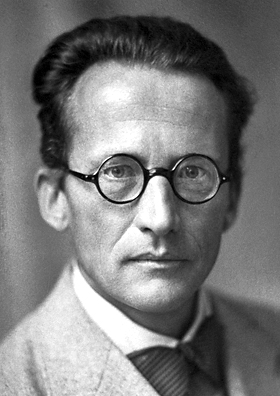
\includegraphics[width=\linewidth]{images/book4/schrodinger-1933.jpg}\par
{\footnotesize Schrödinger in 1933.}
\end{minipage}
\end{history}

\section{Exercises}

\begin{exercise}[$\star$]\label{exo:b3:quantum-model-systems:1}
An electron is confined in a box of length (a) \qty{1.00}{nm}, (b)
\qty{0.50}{nm}. Compute $E_1$ in joules and electronvolts, and the wavelength
of the transition $n = 1 \to 2$.
\end{exercise}

\begin{exercise}[$\star$]\label{exo:b3:quantum-model-systems:2}
List the five lowest levels of a particle in a cubic box, in units of
$h^2/8mL^2$, with their degeneracies.
\end{exercise}

\begin{exercise}[$\star$]\label{exo:b3:quantum-model-systems:3}
Compute the \omterm{def:b3:quantum-model-systems:commutator}{commutators} $[\hat x^2,\hat p]$ and $[\hat p^2,\hat x]$ by acting
on a function $f(x)$.
\end{exercise}

\begin{exercise}[$\star$]\label{exo:b3:quantum-model-systems:4}
% ledger: diat:HCl.Be
With $B = \qty{10.593}{cm^{-1}}$ for \ce{H^{35}Cl}, give the energies (in
\unit{cm^{-1}}) and degeneracies of the levels $J = 0$ to 3, and the moment of
inertia of the molecule.
\end{exercise}

\begin{exercise}[$\star\star$]\label{exo:b3:quantum-model-systems:5}
For the state $\psi_n$ of a \omterm{def:b3:quantum-model-systems:box}{particle in a box}, compute $\langle x\rangle$ and
$\langle x^2\rangle$. Evaluate $\langle x^2\rangle$ for $n = 1$ and compare with
the classical value $L^2/3$ for a particle equally likely to be anywhere.
\end{exercise}

\begin{exercise}[$\star\star$]\label{exo:b3:quantum-model-systems:6}
% ledger: diat:H2.we, diat:D2.we
Compute the harmonic zero-point energies of \ce{H2} and \ce{D2} in
\unit{kJ/mol} from $\tilde\omega_e = \qty{4401.2}{cm^{-1}}$ and
\qty{3115.5}{cm^{-1}}, and their difference. Which ratio of wavenumbers do you
expect from the reduced masses, and how close is the measured one?
\end{exercise}

\begin{exercise}[$\star\star$]\label{exo:b3:quantum-model-systems:7}
The function $\phi = Nx(L - x)$ is a rough guess for the ground state of the
box. Normalise it, then compute its overlap $\langle\psi_1|\phi\rangle$ with
the true ground state.
\end{exercise}

\begin{exercise}[$\star\star$]\label{exo:b3:quantum-model-systems:8}
Show that $\hat p = -\iu\hbar\,\dd/\dd x$ is \omterm{def:b3:quantum-model-systems:hermitian}{Hermitian} for functions that
vanish at the ends of an interval, and that $\hat x\hat p$ is not.
\end{exercise}

\begin{exercise}[$\star\star$]\label{exo:b3:quantum-model-systems:9}
Model hexa-1,3,5-triene as six $\pi$ electrons in a box of length $6l$, $l =
\qty{139.7}{pm}$ (five bonds and half a bond at each end). Predict the
wavelength of its first absorption. Is the molecule coloured?
\end{exercise}

\begin{exercise}[$\star\star\star$]\label{exo:b3:quantum-model-systems:10}
For the model barrier of the figure ($V_0 = \qty{0.40}{eV}$, $a = \qty{50}{pm}$)
at $E = V_0/2$, compute $\kappa$ for a proton and a deuteron and, with the
thick-barrier formula, the ratio $T_H/T_D$. Compare with the exact ratio, 58.
\end{exercise}

\begin{exercise}[$\star\star\star$]\label{exo:b3:quantum-model-systems:11}
Treat the six $\pi$ electrons of benzene as particles on a ring of radius
\qty{139.7}{pm} (the C--C distance equals the radius of a regular hexagon).
Fill the levels, then compute the wavelength of the transition from the
highest filled to the lowest empty level.
\end{exercise}

\begin{exercise}[$\star\star\star$]\label{exo:b3:quantum-model-systems:12}
For the hydrogen $1s$ state, $\psi = (\pi a^3)^{-1/2}\eu^{-r/a}$. Compute the
\omterm{def:b3:quantum-model-systems:hermitian}{expectation value} $\langle r\rangle$ and $\langle V\rangle$, and check that
$\langle V\rangle = 2E_1$. (Use $\int_0^\infty r^n\eu^{-\beta r}\dd r =
n!/\beta^{n+1}$.)
\end{exercise}

\section{Problem: How Long Is a Dye?}

\begin{problem}[{Weekend problem --- the free-electron model of three
cyanine dyes: why a bare chain fails, which transitions are allowed, the
energy scales of a molecule, and the box length that fits}]
\label{pb:b3:quantum-model-systems:1}
% ledger: uvvis:cyanine, uvvis:carbocyanine, uvvis:dicarbocyanine, geo:C6H6.rCC, diat:HCl.we, diat:HCl.Be
Three symmetric cyanine dyes absorb at 524, 603 and 711 nm in ethanol; their
conjugated chains, between and including the two nitrogens, have $j = 5$, 7
and 9 atoms. Take each bond equal to $l = \qty{139.7}{pm}$, $m_e =
\qty{9.109e-31}{kg}$, $h = \qty{6.626e-34}{J.s}$, $c = \qty{2.998e8}{m/s}$,
$k = \qty{1.381e-23}{J/K}$, $\qty{1}{eV} = \qty{1.602e-19}{J}$.

\medskip\noindent\textbf{Part I --- A bare chain.}
\begin{enumerate}
  \item Explain why a chain of $j$ atoms carries $N = j + 1$ $\pi$ electrons, and
        give $N$ for each dye.
  \item Which levels of the box are the highest filled and the lowest empty
        for the first dye?
  \item Show that the first absorption is at $\lambda = 8mcL^2/h(N+1)$.
  \item Give the bare length $L_0 = (j - 1)l$ of each chain.
  \item Compute $\lambda$ for each dye with $L = L_0$.
  \item Compare with the measured values. In which direction is the model
        wrong, and what does that say about $L$?
\end{enumerate}

\medskip\noindent\textbf{Part II --- Which transitions are allowed.}
The intensity of a transition $n \to n'$ is proportional to $|\langle
\psi_n|x - L/2|\psi_{n'}\rangle|^2$.
\begin{enumerate}[resume]
  \item Show that $\psi_n$ is symmetric about the centre of the box for odd
        $n$ and antisymmetric for even $n$.
  \item Deduce that the integral vanishes when $n + n'$ is even.
  \item Is the HOMO $\to$ LUMO transition of each dye allowed?
  \item For the second dye, is the transition from the HOMO to the level
        above the LUMO allowed? From the level below the HOMO to the LUMO?
  \item In the model, at what wavelength (as a fraction of the first one)
        would the next allowed transition from the HOMO lie?
  \item Why does such a rule, derived from symmetry alone, survive the
        crudeness of the model?
\end{enumerate}

\medskip\noindent\textbf{Part III --- The energy scales of a molecule.}
\begin{enumerate}[resume]
  \item Convert the absorption of the second dye into an energy in eV.
  \item The vibration of \ce{HCl} has $\tilde\omega_e = \qty{2991}{cm^{-1}}$:
        convert its quantum into eV.
  \item The rotation of \ce{HCl} has $B = \qty{10.59}{cm^{-1}}$: convert the
        gap between $J = 0$ and $J = 1$ into meV.
  \item Compute $kT$ in meV at \qty{298}{K}.
  \item Which kinds of excitation are populated at room temperature?
  \item In which regions of the spectrum are electronic, vibrational and
        rotational transitions observed?
\end{enumerate}

\medskip\noindent\textbf{Part IV --- The box that fits.}
\begin{enumerate}[resume]
  \item From the measured 603 nm, compute the length $L$ the second dye's
        box must have.
  \item Writing $L = L_0 + 2\delta$, deduce $\delta$.
  \item With this $\delta$, predict $\lambda$ for the first dye; give the
        relative error.
  \item Same question for the third dye.
  \item Interpret $\delta$: where do the $\pi$ electrons go beyond the
        nitrogens?
  \item Express $\delta$ in bond lengths, and state the result of the
        problem: the effective extension of the box at each end.
\end{enumerate}
\end{problem}
